\documentclass[12pt]{article}
\usepackage[margin=2.5cm]{geometry}
\usepackage{enumerate}
\usepackage{amsfonts}
\usepackage{amsmath}
\usepackage{fancyhdr}
\usepackage{amsmath}
\usepackage{amssymb}
\usepackage{amsthm}
\usepackage{mdframed}
\usepackage{graphicx}
\usepackage{subcaption}
\usepackage{adjustbox}
\usepackage{listings}
\usepackage{xcolor}
\usepackage{courier}
\usepackage[utf]{kotex}
\usepackage{hyperref}
\usepackage{soul}

\definecolor{codegreen}{rgb}{0,0.6,0}
\definecolor{codegray}{rgb}{0.5,0.5,0.5}
\definecolor{codepurple}{rgb}{0.58,0,0.82}
\definecolor{backcolour}{rgb}{0.95,0.95,0.92}

\lstdefinestyle{mystyle}{
    backgroundcolor=\color{backcolour},
    commentstyle=\color{codegreen},
    keywordstyle=\color{magenta},
    numberstyle=\tiny\color{codegray},
    stringstyle=\color{codepurple},
    basicstyle=\ttfamily\footnotesize,
    breakatwhitespace=false,
    breaklines=true,
    captionpos=b,
    keepspaces=true,
    numbers=left,
    numbersep=5pt,
    showspaces=false,
    showstringspaces=false,
    showtabs=false,
    tabsize=1
}

\lstset{style=mystyle}

\pagestyle{fancy}
\renewcommand{\headrulewidth}{0.4pt}
\lhead{CSC 369}
\rhead{Midterm 2 Notes}

\begin{document}
\title{CSC 369 Midterm 2 Notes}

\section{Virtualizing CPU}

\begin{itemize}
    \item Turns a single CPU into a seemingly infinite number of CPUS, and
    allows many programs to seemingly run at once
    \item To implement CPU virtualization, the OS needs low-level machinery
    called \textbf{mechanism} and high level intelligence called \textbf{policies}
    \item Steps

    \begin{enumerate}[1.]
        \item Involve OS to setup hardware hardwre to limit what the process can do without OS assistance
        (\textbf{Limited Direct Execution})

        \bigskip

        This is done so by

        \bigskip

        \begin{enumerate}[1.]
            \item Setting up trap handler
            \item Starting an interrupt timer (so process won't last forever)
        \end{enumerate}
        \item Involve OS to intervene at key points to perform previleged operations
        or switch out operations when they have monopolized the CPU too long
    \end{enumerate}
    \bigskip
\end{itemize}

\section{Limited Direct Execution}

\begin{itemize}
    \item Idea: Just run the program you want to run on the CPU,
    but first make sure to set up the hardware so as to limit what
    process can do without OS assistance
    \item baby proofs the CPU by

    \bigskip

    \begin{enumerate}[1.]
        \item Setting up trap handlers
        \item Starts an interrupt timer
        \item Run processes in a restricted mode
    \end{enumerate}

    \bigskip

    \underline{\textbf{Example}}

    \bigskip

    Baby proofing a room:

    \bigskip

    \begin{itemize}
        \item Locking cabinets containing dangerous stuff and covering electrical sockets.
        \item When room is readied, let your baby roam free in knowledge that all the dangerous
        aspect of the room is restricted
    \end{itemize}
\end{itemize}

\section{Trap Handlers}

\begin{itemize}
    \item Is instruction that tells the hardware what to run when certain exceptions occur

    \bigskip

    \underline{\textbf{Example}}

    \bigskip

    What code to run when

    \begin{enumerate}[1.]
        \item Hard disk interrupt occurs
        \item Keyboard interrupt occrs
        \item Program makes a system call?
    \end{enumerate}

\end{itemize}

\section{Timer Interrupt}

\begin{itemize}
    \item Is a hardware mechanism that ensures the user program does not run forever
    \item Is emitted at regular intervals by a timer chip $^{[6]}$
\end{itemize}

\section{Response Time}
\begin{itemize}
    \item \textbf{Formula} $T_{response} = T_{firstrun} - T_{arrival}$
    \item measures the interactive performance between users and the system
\end{itemize}

\section{Turnaround Time}

\begin{itemize}
    \item \textbf{Formula} $T_{turnaround} = T_{completion} - T_{arrival}$
    \item measures the amount of time taken to complete a process
\end{itemize}

\section{Starvation}

\begin{itemize}
    \item Is the problem that occurs when high priority processes keep
    executing and low priority processes get blocked for indefinite time $^{[1]}$
\end{itemize}

\section{Convoy Effect}

\begin{itemize}
    \item Is the problem where number of relatively-short potential consumers
    of a resource get queued behind a heavy weight consumer

    \bigskip

    \begin{center}
    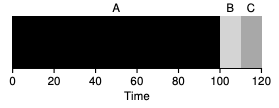
\includegraphics[width=0.7\linewidth]{images/midterm_2_solution_5.png}
    \end{center}
\end{itemize}

\section{Scheduling policies}

\begin{itemize}
    \item Are algorithms for allocating CPU resources to concurrent tasks
    deployed on (i.e., allocated to) a processor (i.e., computing resource)
    or a shared pool of processors $^{[5]}$
    \item Are sometimes called \textbf{Discipline}
    \item Covers the following algorithms in textbook

    \begin{itemize}
        \item \textbf{First In First Out}

        \begin{itemize}
            \item Is the most basic scheduling algorithm
            \item Is vulnerable to \textbf{convoy effect}
            \item No \textbf{starvation} as long as every process eventually completes
        \end{itemize}

        \item \textbf{Shortest Job First}

        \begin{itemize}
            \item Improves average \textbf{turnaround time} given processes of uneven length
            \item Is a general scheduling principle useful in situation where turnaround time
            per process matters
            \item Is vulnerable to \textbf{convoy effect}

            \begin{center}
            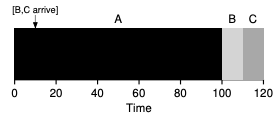
\includegraphics[width=0.7\linewidth]{images/midterm_2_solution_6.png}
            \end{center}

            \item Is vulnerable to \textbf{starvation}
            \begin{itemize}
                \item When only short-term jobs come in while a long term job is in queue
            \end{itemize}
        \end{itemize}
        \item \textbf{Shortest Time-to-completion First}

        \begin{itemize}
            \item Addresses \textbf{convoy effect} in \textbf{Shortest Job First}
            \item Determines which of the remaining+new jobs has least time left, and
            schedule accordingly at \underline{any time}

            \bigskip

            \begin{center}
            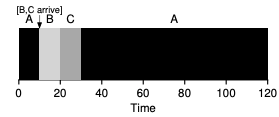
\includegraphics[width=0.7\linewidth]{images/midterm_2_solution_7.png}
            \end{center}

            \item Is vulnerable to \textbf{starvation}
            \begin{itemize}
                \item When only short-term jobs come in while a long term job is in queue
            \end{itemize}

        \end{itemize}

        \item \textbf{Round Robin}

        \begin{itemize}
            \item Has good \textbf{response time} but terrible \textbf{turnaround time}
            \item Runs job for a \textbf{time slice} or \textbf{quantum}
            \item Each job gets equal share of CPU time
            \item Is clock-driven $^{[6]}$
            \item Is starvation-free $^{[7]}$
            \item \underline{Must} have the length of a time slice (\textbf{quantum}) as multiple of timer-interrupt period
        \end{itemize}

        \bigskip

        \begin{center}
        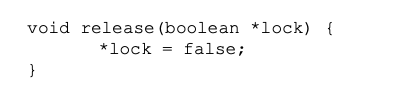
\includegraphics[width=0.7\linewidth]{images/midterm_2_solution_4.png}
        \end{center}
        \item \textbf{Multi-level Feedback Queue}

        \begin{itemize}
            \item Is the most well known approaches to shceduling
            \item Optimizes \textbf{turnaround time}, and minimizes \textbf{response time}
            \item Observees the execution of a job and priortizes accordingly without prior knowledge
            \item Rules

            \begin{itemize}
                \item \textbf{Rule 1:} If Priority(A) $>$ Priority(B), A runs (B doesn't)
                \item \textbf{Rule 2:} If Priority(A) $=$ Priority(B). A \& B run in round-robin
                fashion using the time slice (quantum length) of the given queue
                \item \textbf{Rule 3:} When a job enters the system, it is placed at the highest
                priority(the top most queue)
                \item \textbf{Rule 4:} Once a job uses up its time allotment at a given level
                (regardless of how many times it has given up the CPU), its priority is reduced
                (it moves down on queue)
                \item \textbf{Rule 5:} After some time period S, move all the jobs in the system to the
                topmost queue.
            \end{itemize}

            \bigskip

            \begin{center}
            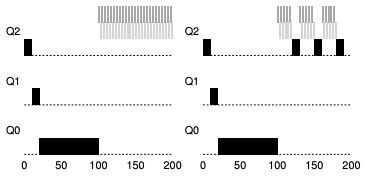
\includegraphics[width=0.7\linewidth]{images/midterm_2_solution_8.png}
            \end{center}
        \end{itemize}
    \end{itemize}
\end{itemize}

\section{User Mode}

\begin{itemize}
    \item Is restricted
    \item Executing code has no ability to \textit{directly} access
    hardware or reference memory $^{[1]}$
    \item Crashes are always recoverable $^{[1]}$
    \item Is where most of the code on our computer / applications are executed $^{[3]}$
\end{itemize}

\section{Kernel Mode}
\begin{itemize}
    \item Is previleged (non-restricted)
    \item Executing code has complete and unrestricted access to the underlying hardware $^{[3]}$
    \item Is generally reserved for the lowest-level, most trusted functions of the operating
    system $^{[1]}$
    \item Is fatal to crash; it will halt the entire PC (i.e the blue screen of death) $^{[3]}$
\end{itemize}

\section{Interrupt}

\begin{itemize}
    \item i is a signals are sent by hardware (keyboardm mouse, etc.), or software (page fault, protection violation, system call)
    \item Tells the CPU to stop its current activities and execute the appropriate part of the operating system (\textbf{Interrupt Handler}). $^{[2]}$
    \item Has three different types $^{[2]}$

    \begin{enumerate}[1)]
        \item \textbf{Hardware Interupts}

        \begin{itemize}
            \item Are generated by hardware devices to signal that they need some attention from the OS.
            \item May be due to receiving some data

            \bigskip

            \underline{\textbf{Examples}}

            \bigskip

            \begin{itemize}
                \item Keystrokes on the keyboard
                \item Receiving data on the ethernet card
            \end{itemize}

            \bigskip

            \item May be due to completing a task which the operating system previous requested

            \bigskip

            \underline{\textbf{Examples}}

            \bigskip

            Transfering data between the hard drive and memory
        \end{itemize}

        \bigskip

        \item \textbf{Software Interupts}

        \bigskip

        \begin{itemize}
            \item Are generated by programs when a system call is requested
        \end{itemize}

        \bigskip

        \item \textbf{Traps}

        \bigskip

        \begin{itemize}
            \item Are generated by the CPU itself
            \item Indicate that some error or condition occured for which assistance from the operating system is needed
        \end{itemize}

        \bigskip
    \end{enumerate}
\end{itemize}

\section{Content Switch}

\begin{itemize}
    \item Is switching from running a user level process to the OS kernel and often
    to other user processes before the current process is resumed
    \item Happens during a timer interrupt or system call
    \item Saves the following states for a process during a context switch
    \begin{itemize}
        \item Stack Pointer
        \item Program Counter
        \item User Registers
        \item Kernel State
    \end{itemize}
    \item May hinder performance
\end{itemize}

\section{System Call}

\bigskip

\begin{itemize}
    \item Is the programmatic way in which a computer program requests a previleged service from the kernel of the operating system
    \item i.e. Reading from disk
    \item Is strictly a subset of software interrupts
    \item Steps

    \begin{enumerate}[1)]
        \item Setup \textbf{trap tables} on boot
        \item Execute system call
        \item Save \textit{Program Counter}, \textit{CPU registers}, \textit{kernal stack} (so process can resume after \textbf{return-from-trap}
        or \textbf{context switch})
        \item Switch from \textbf{user mode} to \textbf{kernel mode}
        \item Perform previleged operations
        \item Finish and execute \textbf{return-from-trap} instruction
        \item Return from \textbf{kernel mode} to \textbf{user mode} and resume user program
    \end{enumerate}
\end{itemize}

\underline{\textbf{Example}}

\begin{itemize}
    \item \texttt{yield()}
    \begin{itemize}
        \item Is a system call
        \item Causes the calling thread to relinquish the CPU
        \item Places the current thread at the end of the run queue
        \item Schedules another thread to run
    \end{itemize}
\end{itemize}

\section{Signals}

\begin{itemize}
    \item Provides a way to communicate with the process
    \item Can cause job to stop, continue, or terminate
    \item Can be delivered to an application

    \begin{itemize}
        \item Stops the application from whatever its doing
        \item Runs Signal handler (some code in application to handle the signal)
        \item When finished, the process resumes previous behavior
    \end{itemize}
\end{itemize}

\section{CPU-bound process} $^{[8]}$

\begin{itemize}
    \item CPU Bound processes are ones that are implementing algorithms
    with a large number of calculations
    \item Programs such as simulations may be CPU bound for most of the life of the process.
    \item Users do not typically expect an immediate response from the computer when running CPU bound programs.
    \item They should be given a lower priority by the scheduler.
\end{itemize}
\section{I/O-bound process} $^{[8]}$

\begin{itemize}
    \item Processes that are mostly waiting for the completion of input or output (I/O) are I/O Bound.
    \item Interactive processes, such as office applications are mostly I/O bound the entire life of the process. Some processes may be I/O bound for only a few short periods of time.
    \item The expected short run time of I/O bound processes means that they will not stay the running the process for very long.
    \item They should be given high priority by the scheduler.
\end{itemize}

\section{Virtualizing Memory}
\begin{itemize}
    \item Basic Idea: For the most part, let the program run directly on the hardware;
    however, at certain key points in time (e.g. system call, timer interrupt), arrange
    so that the OS gets involved and make sure the 'Right' thing happens.
    \item Like CPU, many programs are sharing the memory at the same time
    \item Like CPU, the goal is to create an illusion that it has its own code and data
    \item Like CPU, the memory also needs low-level machinery called \textbf{mechanism},
    and high level intelligence called \textbf{policies}
    \item Steps

    \begin{enumerate}[1.]
        \item Use \textbf{address translation} to transform each memory access,
        changing \textbf{virtual address} provided by instruction to \textbf{physical address}
        \begin{itemize}
            \item Memory access includes instruction fetch, load, or store
            \item Is done using hardware
        \end{itemize}
        \item Invove OS at key points to \textbf{manage memory}

        \bigskip

        Memory management includes

        \bigskip

        \begin{enumerate}[1.]
            \item Setting up hardware so correct translations take place
            \item Keeping track of which locations are free and which are in use
            \item Judiciously intervening to maintain control over how memory is used
        \end{enumerate}

        \bigskip
    \end{enumerate}
\end{itemize}

\section{Address Translation}

\begin{itemize}
    \item Is also called \textbf{hardware-based address translation}
    \item Is a mechanism of memory virtualization
    \item Is the technique of transforming virtual address to physical address
\end{itemize}

\pagebreak

\section{Critical Section}

\begin{itemize}
    \item Is a piece of code that accesses a \textit{shared} resource,
    \ul{usually a variable or data structure}
\end{itemize}

\section{Thread}

\begin{itemize}
    \item Is a lightweight process that can be managed independently by a schdeduler $^{[4]}$
    \item Improves the application performance using parallelism. (e.g peach)

    \begin{center}
    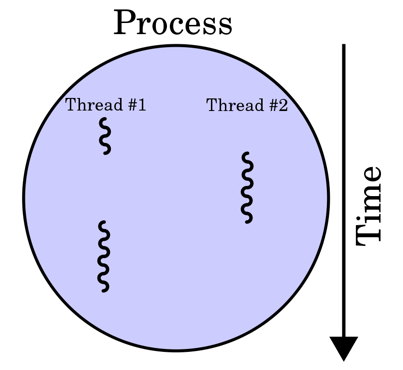
\includegraphics[width=0.4\linewidth]{images/midterm_2_solution_1.png}
    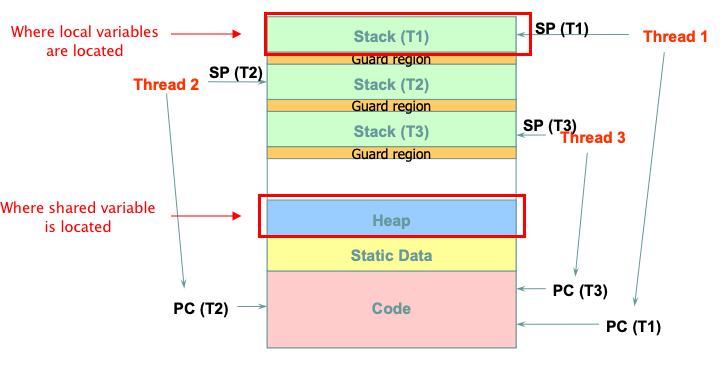
\includegraphics[width=\linewidth]{images/midterm_2_solution_2.png}
    \end{center}

    \item A thread is bound to a single process
    \item A process can have multiple threads
    \item Has two types
    \begin{itemize}
        \item \textbf{User-level Threads:}

        \begin{itemize}
            \item Are implemented by users and kernel is not aware of the existence of these threads
            \item Are represented by a program counter(PC), stack, registers and a small process control block
            \item Are small and much faster than kernel level threads
        \end{itemize}
        \item \textbf{Kernel-level Threads:}

        \begin{itemize}
            \item Are handled by the operating system directly
            \item Thread management is done by the kernel
            \item Are slower than user-level threads
        \end{itemize}
    \end{itemize}
\end{itemize}

\section{Thread API}

\begin{itemize}

    \item \texttt{pthread\_create}

    \begin{itemize}
        \item \textbf{syntax:}

        \bigskip
\begin{lstlisting}[language=c]
int pthread_create(pthread_t *thread,
               const pthread_attr_t *attr,
               void * (*start_routine)(void*),
               void * arg)
\end{lstlisting}

        \begin{itemize}
            \item \texttt{thread}

            \begin{itemize}
                \item is a pointer to a structure of type \texttt{pthread\_t}
            \end{itemize}
            \item \texttt{attr}

            \begin{itemize}
                \item is used to specify any attributes this thread might have
                \item is initialized with a separate call \texttt{pthread\_attr\_init()}
                \item set default by passing \texttt{NULL}
            \end{itemize}

            \item \texttt{(start\_routine)}

            \begin{itemize}
                \item means which function this thread should start running in?
                \item setting void pointer \texttt{(void *)} as an argument to function \texttt{start\_routine}
                allows us to pass in \underline{any} type of argument
                \item setting void pointer \texttt{(void *)} as return type allows us to return
                \underline{any} type of result
            \end{itemize}

            \item \texttt{args}

            \begin{itemize}
                \item is where to pass the arguments for the function pointer \texttt((start\_routine))
            \end{itemize}

            \bigskip

            \underline{\textbf{Example}}

            \begin{center}
            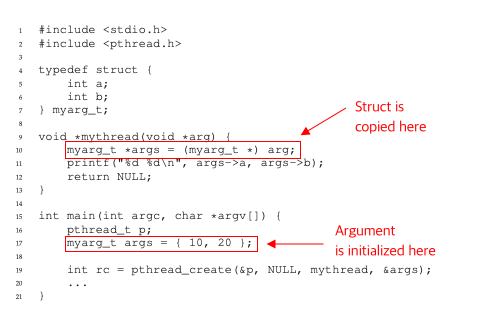
\includegraphics[width=\linewidth]{images/midterm_2_solution_19.png}
            \end{center}
        \end{itemize}
    \end{itemize}

    \item \texttt{pthread\_cond\_wait}

    \begin{itemize}
        \item Puts the calling thread to sleep (a blocked state)
        \item Waits for some other thread to signal it
    \end{itemize}

    \bigskip

    \underline{\textbf{Example}}

    \begin{center}
    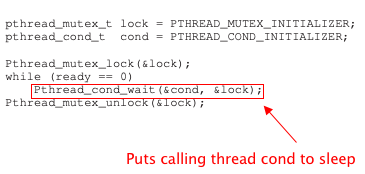
\includegraphics[width=0.7\linewidth]{images/midterm_2_solution_9.png}
    \end{center}

    \item \texttt{pthread\_cond\_signal}

    \begin{itemize}
        \item Is used to \underline{unblocks at least one} of the threads that
        are blocked on the specified condition variable cond
    \end{itemize}

    \bigskip

    \underline{\textbf{Example}}

    \begin{center}
    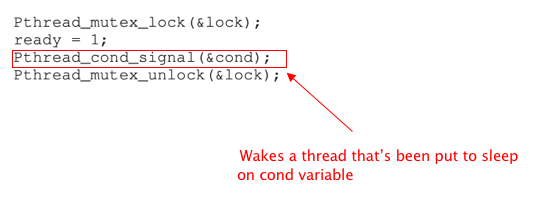
\includegraphics[width=0.8\linewidth]{images/midterm_2_solution_10.png}
    \end{center}

\end{itemize}

\section{Condition Variable}

\begin{itemize}
    \item is an explicit queue that threads can put themselves on when some
    state of execution is not as desired (so it can be put to sleep)
    \item when states are changed, one or more of the waiting threads can be
    awaken and be allowed to continue (done by \textbf{signaling} the condition)
    \item queue is \textbf{FIFO}
    \item \texttt{wait()} call is used to put thread to sleep
    \item \texttt{singal()} call is used to awake thread from sleep
    \item \textbf{Syntax (initialization):}

    \bigskip

    \texttt{pthread\_cont\_t c = PTHREAD\_COND\_INITIALIZER}

    \bigskip

    \underline{\textbf{Example}}

    \begin{center}
    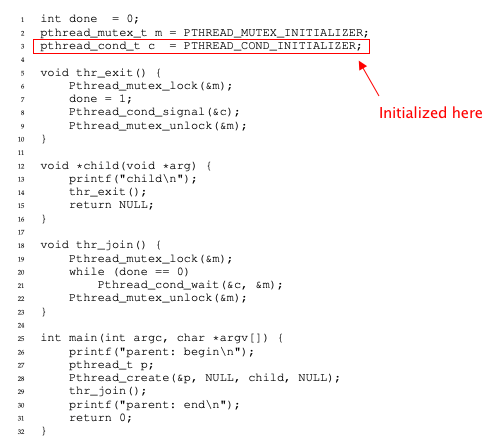
\includegraphics[width=\linewidth]{images/midterm_2_solution_16.png}
    \end{center}

    \item

    \textbf{Syntax (Wait):}

    \bigskip

    \texttt{Pthread\_cond\_wait(pthread\_cond\_t *c, pthread\_mutex\_t *m)}

    \bigskip

    \underline{\textbf{Example}}

    \begin{center}
    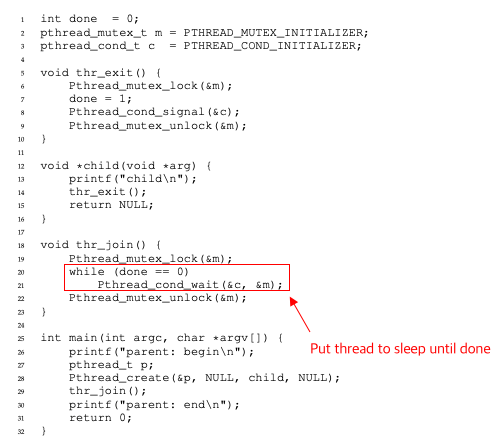
\includegraphics[width=\linewidth]{images/midterm_2_solution_17.png}
    \end{center}
    \item \textbf{Syntax (Signal):}

    \bigskip

    \texttt{Pthread\_cond\_signal(pthread\_cond\_t *c)}

    \underline{\textbf{Example}}

    \begin{center}
    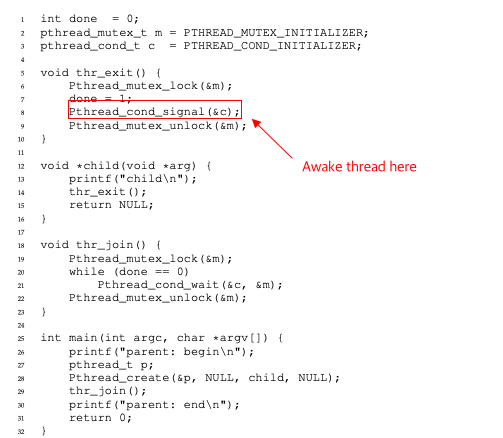
\includegraphics[width=\linewidth]{images/midterm_2_solution_18.png}
    \end{center}

\end{itemize}

\section{Spinlock}
\begin{itemize}
    \item Is the simplest lock to build
    \item Uses a lock variable

    \begin{itemize}
        \item 0 - (available/unlock/free)
        \item 1 - (acquired/locked/held)
    \end{itemize}

    \item Has two operations

    \begin{enumerate}[1.]
        \item \texttt{acquire()}

        \bigskip

        \begin{center}
        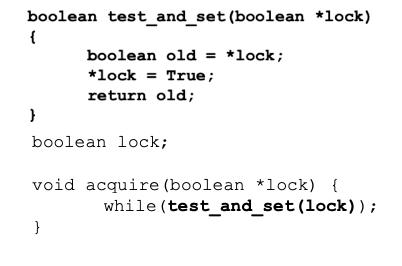
\includegraphics[width=0.7\linewidth]{images/midterm_2_solution_3.png}
        \end{center}

        \bigskip

        \item \texttt{release()}

        \bigskip

        \begin{center}
        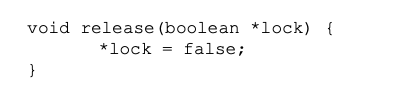
\includegraphics[width=0.7\linewidth]{images/midterm_2_solution_4.png}
        \end{center}

        \bigskip
    \end{enumerate}
    \item Allows a single thread to enter critical section at a time
    \item Spins using CPU cycles until the lock becomes available.
    \item May spin forever
\end{itemize}

\section{Livelock}

\begin{itemize}
    \item Two or more threads reapeatedly attempting this code over and over (e.g acquiring lock), but progress is
    not being made (e.g acquiring lock)
    \item Solution: Add a random delay before trying again (decrease odd of livelock)
\end{itemize}

\section{Deadlock}

\begin{center}
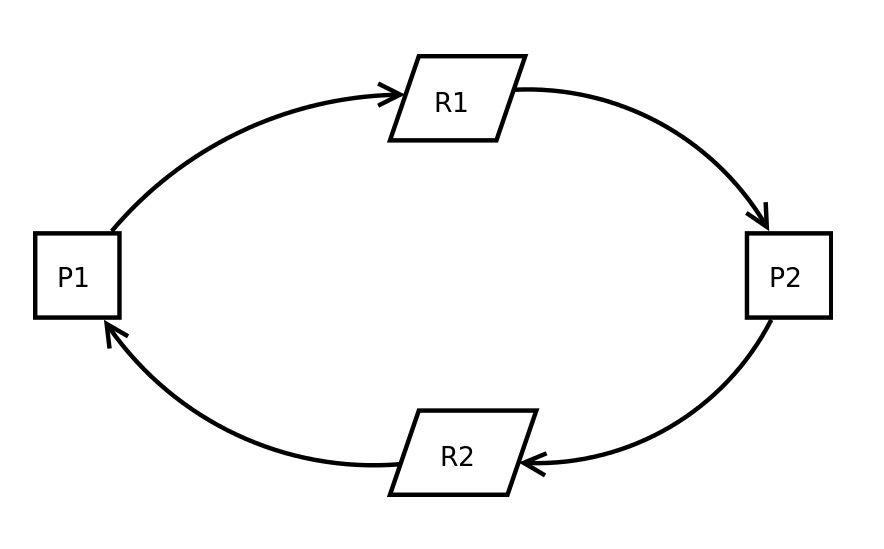
\includegraphics[width=0.6\linewidth]{images/midterm_2_solution_11.png}
\end{center}

\begin{itemize}
    \item Is a state in which each member of a group is waiting for
    another member including itself, to take action (e.g. releasing lock)
    \item Conditions for Deadlock (All four must be met)

    \begin{itemize}
        \item \textbf{Mutual Exclusion}
        \begin{itemize}
            \item Occurs when threads claim exclusive control of resources that
            they require (e.g. thread grabing a lock)
        \end{itemize}
        \item \textbf{Hold-and-wait}
        \begin{itemize}
            \item Occurs when threads hold resources allocated to them (e.g locks that they have already acquired)
            while waiting for additional resources (e.g. locks that they wish to acquire)
        \end{itemize}

        \item \textbf{No Preemption}
        \begin{itemize}
            \item Occurs when resource cannot be forcibly removed from threads that are holding them
        \end{itemize}
        \item \textbf{Circular Wait}
        \begin{itemize}
            \item Occurs when there exists a circular chain of threads such that
            each threads hold one or more resources (e.g. locks) that are being
            requested by the next thread in the chain.
        \end{itemize}
    \end{itemize}

    \bigskip

    \underline{\textbf{Example}}

    \begin{center}
    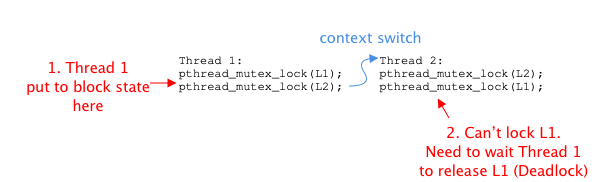
\includegraphics[width=0.9\linewidth]{images/midterm_2_solution_12.png}
    \end{center}

    \item Preventions

    \begin{itemize}
        \item \textbf{Circular Wait}
        \begin{itemize}
            \item Write code such that circular wait is never induced
            \item Is the most practical prevention technique
            \item Requires deep understanding of the code base
            \item \textbf{Total Ordering} (Most starightforward)

            \bigskip

            \underline{\textbf{Example}}

            \bigskip

            Given two locks in the system (\texttt{L1} and \texttt{L2}), always
            acuiqure \texttt{L1} before \texttt{L2}

            \bigskip

            \item \textbf{Partial Ordering} (Applied to complex systems)

            \bigskip

            \underline{\textbf{Example}}

            \bigskip

            Memory mapping code in Linux (has then different groups).

            \bigskip

            (Simple) \texttt{i\_mutex} before \texttt{i\_mmap\_mutex}

            \bigskip

            (More complex) \texttt{i\_mmap\_mutex} before \texttt{private\_lock}
            before \texttt{swap\_lock} before \texttt{mapping->tree\_lock}

        \end{itemize}

        \item \textbf{Hold-and-wait}
        \begin{itemize}
            \item Can be avoided by acquiring all locks at once
            \item Can be problematic
            \item Must know which lock must be held and acquire ahead of time
            \item Is likely to decrease concurrency (since all need to be acquired over their needs)

            \bigskip

            \underline{\textbf{Example}}

            \bigskip

            \begin{center}
            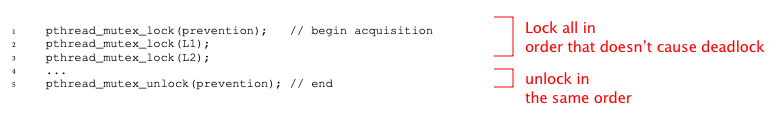
\includegraphics[width=\linewidth]{images/midterm_2_solution_13.png}
            \end{center}
        \end{itemize}

        \item \textbf{No Preemption}
        \begin{itemize}
            \item Can be avoided by adding code that force unlock if not available

            \begin{center}
            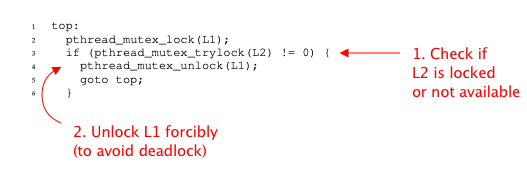
\includegraphics[width=0.8\linewidth]{images/midterm_2_solution_14.png}
            \end{center}

            \item \texttt{pthread\_mutex\_trylock} tries to lock the speicied mutex.
            \item \texttt{pthread\_mutex\_trylock} returns 0 if lock is available
            \item \texttt{pthread\_mutex\_trylock} returns the following error if occupied

            \bigskip

            \quad \texttt{EBUSY} - Mutex is already locked

            \bigskip

            \quad \texttt{EINVAL} - Is not initialized mutex

            \bigskip

            \quad \texttt{EFAULT} - Is in valid pointer

            \item May result in \textbf{live lock}
        \end{itemize}

        \item \textbf{Mutual Exclusion}
        \begin{itemize}
            \item Idea: Avoid the mutual exclusion at all
            \item Use \textbf{lock-free}/\textbf{wait-free} approach:
            building data structures in a manner that does not require explicit locking
            using hardware instructions

            \bigskip

            \underline{\textbf{Example}}

            \bigskip

            \begin{center}
            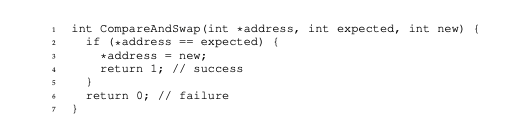
\includegraphics[width=\linewidth]{images/midterm_2_solution_15.png}
            \end{center}

        \end{itemize}
    \end{itemize}

    \item Avoidance

    \begin{itemize}
        \item \textbf{Banker's Algorithm}
    \end{itemize}
\end{itemize}

\section{Process}

\begin{itemize}
    \item Is a program in execution
    \item Is named by it's process ID or PID
    \item Can be described by the following states at any point in time

    \begin{itemize}
        \item Address Space
        \item CPU Registers
        \item Program Counter
        \item Stack Pointer
        \item I/O Information
    \end{itemize}

    (wait. this is PCB)

    \item Exists in one of many different \textbf{process states}, including

    \begin{enumerate}[1.]
        \item Running
        \item Ready to Run
        \item Blocked
    \end{enumerate}

    \bigskip

    \begin{itemize}
        \item Different events (Getting Scheduled, descheduled, or waiting for I/O)
        transitions one of these states to the other
    \end{itemize}

\end{itemize}

\bigskip

\underline{\textbf{References}}

\begin{enumerate}[1)]
    \item Coding Horror, Understanding User and Kernel Mode, \href{https://blog.codinghorror.com/understanding-user-and-kernel-mode/}{link}
    \item Kansas State University, Basics of How Operating Systems Work, \href{http://faculty.salina.k-state.edu/tim/ossg/Introduction/OSworking.html#:~:text=Interrupts%20are%20signals%20sent%20to,part%20of%20the%20operating%20system.&text=Hardware%20Interupts%20are%20generated%20by,some%20attention%20from%20the%20OS.}{link}
    \item Kansas State University, Glossary, \href{http://faculty.salina.k-state.edu/tim/ossg/glossary.html#term-context-switch}{link}
    \item Tutorials Point, User-level threads and Kernel-level threads, \href{https://www.tutorialspoint.com/user-level-threads-and-kernel-level-threads}{link}
    \item Science Direct, Scheduling Policy, \href{https://www.sciencedirect.com/topics/computer-science/scheduling-policy#:~:text=Scheduling%20policies%20are%20algorithms%20for,nature%20of%20applications%20%5B1%5D.}{link}
    \item Guru 99: What is CPU Scheduling?, \href{https://www.guru99.com/cpu-scheduling-algorithms.html#8}{link}
    \item Wikipedia: Round-robin Scheduling, \href{https://en.wikipedia.org/wiki/Round-robin_scheduling}{link}
    \item Kansas State University, The Process Scheduler, \href{http://faculty.salina.k-state.edu/tim/ossg/Process/scheduler/scheduler.html#:~:text=CPU%20Bound%20processes%20are%20ones,the%20life%20of%20the%20process.}{link}
\end{enumerate}

\pagebreak

\section*{Index-based File System}

\begin{center}

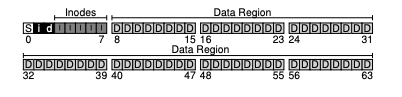
\includegraphics[width=\linewidth]{images/midterm_2_solution_20.png}
\end{center}

\begin{itemize}
    \item Has following parts

    \begin{itemize}
        \item Superblock
        \item Inode Bitmap
        \item Data Bitmap
        \item Inodes
        \item Data Region
    \end{itemize}

    \item Each block in file system is 4KB
    \item Uses a large amount of metadata per file (especially for large files)
\end{itemize}

\section*{Superblock}

\begin{center}
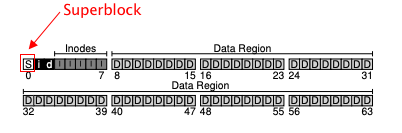
\includegraphics[width=\linewidth]{images/midterm_2_solution_21.png}
\end{center}

\begin{itemize}
    \item contains information about the file system, including

    \begin{enumerate}[1.]
        \item the number of inodes and data blocks in a particular file system
        \item the magic number of some kind to identify the file system type (e.g NFS, FFS, VSFS)
    \end{enumerate}

    \item The OS reads superblock \underline{first} to initialize various parameters,
    and then attach volume to the file-system tree
\end{itemize}

\section*{Bitmap}

\begin{center}
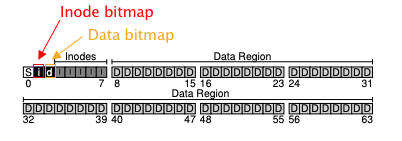
\includegraphics[width=\linewidth]{images/midterm_2_solution_22.png}
\end{center}

\begin{itemize}
    \item Tracks whether inode or data blocks are free or allocated
    \item Is a simple and popuar structure
    \item Uses each bit
    \begin{itemize}
        \item \texttt{0} means free
        \item \texttt{1} means in use
    \end{itemize}

    \item \textbf{Data Bitmap} is bitmap for data region
    \item \textbf{Inode Bitmap} is bitmap for inode region
\end{itemize}

\section*{Inode}

\begin{center}
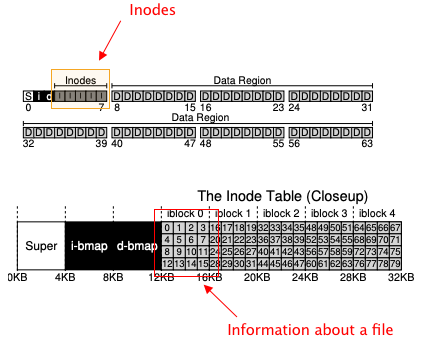
\includegraphics[width=\linewidth]{images/midterm_1_solution_12.png}
\end{center}

\begin{itemize}
    \item Is a short form for \textbf{index node}
    \item Contains disk block location of the object's data $^{[7]}$
    \item Contains all the information you need about a file (i.e. metadata)

    \begin{itemize}
        \item File Type
        \begin{itemize}
            \item e.g. regular file, directory, etc
        \end{itemize}
        \item Size
        \item Number of blocks allocated to it
        \item Protection information
        \begin{itemize}
            \item such as who owns the file, as well as who can access it
        \end{itemize}
        \item Time information
        \begin{itemize}
            \item e.g. When file was created, modified, or last accessed
        \end{itemize}
        \item Location of data blocks reside on disk
    \end{itemize}
\end{itemize}

\section*{Data Region}

\begin{center}
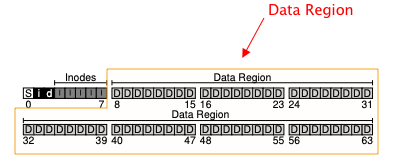
\includegraphics[width=\linewidth]{images/midterm_1_solution_11.png}
\end{center}

\begin{itemize}
    \item Is the region of disk we use for user data
\end{itemize}


\section{Block}

\begin{itemize}
    \item Size of each block is 4KB
\end{itemize}

\section{lseek}

\begin{itemize}
    \item \textbf{Syntax:} \texttt{off\_t lseek(int fildes, off\_t offset, int whence)}

    \begin{itemize}
        \item \texttt{fildes} - file descriptor
        \item \texttt{offset} - file offset to a particular position in file
    \end{itemize}
\end{itemize}

\section{Kilobyte}

\begin{itemize}
    \item 1 kilobyte is \underline{1024 bytes}
\end{itemize}

\section{file}
\begin{itemize}
    \item is an array of bytes which can be created, read, written and deleted
    \item low-level name is called \textbf{inode number} or \textbf{i-number}
\end{itemize}
\section{Reading a File From Disk}

\bigskip

\underline{\textbf{Example}}

\bigskip

When

\bigskip

\texttt{open("/foo/bar", O\_READONLY)}

\bigskip

is called

\bigskip

\begin{itemize}
    \item the goal is to find the inode of the file \texttt{bar} to read its basic information
    (i.e. includes permission, information, file size etc)
    \item done by traversing the pathname and locate the desired inode
    \item Steps

    \begin{enumerate}[1.]
        \item Begin traversal at the root of the file system, in the \textbf{root directory}

        \item Find \textbf{inode} of the root directory by looking for \texttt{i-number}

        \begin{itemize}
            \item \textbf{i-number} is found in it's parent directoy
            \item for root directory, there is no parent directory
            \item it's inode number is 2 (for UNIX file systems)
        \end{itemize}

        \item Read the \textbf{inode} of root directory
        \item Once its \textbf{inode} is read, look inside to find pointers
        to data blocks
        \item Recursively traverse the pathname until the desired inode is found (e.g \texttt{foo} $\to$ \texttt{bar})
        \item Issue a \texttt{read()} system call to read from file

        \begin{itemize}
            \item \texttt{fd} with offset \texttt{0} reads the first file block (e.g. \texttt{bar data[0]})
            \item \texttt{lseek(..., offset\_amt * size\_of\_file\_block)} is used to offset/move to desired block in \texttt{bar}
        \end{itemize}

        \item Trasnfer data to \texttt{buf} data block

        \item Close \texttt{fd}. No I/O is read.
    \end{enumerate}
\end{itemize}

\section{inode}

\begin{itemize}
    \item total size may vary
    \item inode pointer has size of 4 byte
    \item Has 12 \textbf{direct pointers} to 4KB data blocks
    \item Has 1 \textbf{indirect pointer} [when file grows large enough]
    \item Has 1 \textbf{double indirect Pointer} [when file grows large enough]
    \item Has 1 \textbf{triple indirect Pointer} [when file grows large enough]
\end{itemize}

\section{Indirect Pointers}

\begin{itemize}
    \item Is allocated to data-block if file grows large enough
    \item Has total size of 4 KB or 4096 bytes
    \item Has $4096/4 = 1024$ pointers
    \item Each pointer points to 4KB data-block
    \item File can grow to be $(12 + 1024) \times 4\text{K} = 4144\text{KB}$
\end{itemize}

\section{Double Indirect Pointers}

\begin{itemize}
    \item is allocated when single indirect pointer is not large enough
    \item each pointer in first pointer block points to another pointer block
    \item has $1024^2$ pointers
    \item each of $1024^2$ pointers point to 4KB data block
    \item File can grow to be $(12 + 1024 + 1024^2) \times 4\text{K} = 4198448\text{KB}$ or $\approx 4.20 \text{GB}$

    \begin{center}
    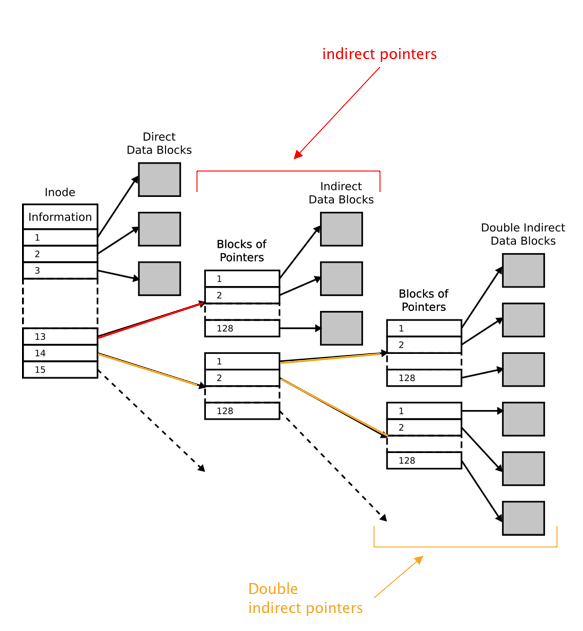
\includegraphics[width=\linewidth]{images/midterm_1_solution_13.png}
    \end{center}
\end{itemize}

\section{Triple Indirect Pointers}

\begin{itemize}
    \item is allocated when double indirect pointer is not large enough
    \item has $1024^3$ pointers
    \item each of $1024^3$ pointers point to 4KB data block
    \item File can grow to be $(12 + 1024 + 1024^2 + 1024^3) \times 4\text{K} = 4299165744\text{KB}$ or $\approx 4.00 \text{TB}$
\end{itemize}

\section{Old UNIX File system}
\begin{itemize}
    \item was simple, and looked like the following on disk

    \begin{center}
    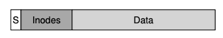
\includegraphics[width=0.6\linewidth]{images/midterm_1_solution_16.png}
    \end{center}
    \item has terrible performance
    \item suffers from \textbf{external fragmentation}
    \item had small data block (512 bytes) and transfer of data took too long
\end{itemize}

\section{Fast File System}

\begin{itemize}
    \item modern file system has same APIS (\texttt{read()}, \texttt{write()}, \texttt{open()}, \texttt{close()})
    \item divides into a number of \textbf{cylinder groups}

    \begin{center}
    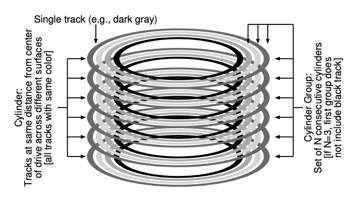
\includegraphics[width=0.8\linewidth]{images/midterm_1_solution_17.png}
    \end{center}
    \item each \textbf{block group} or \textbf{cylinder group} is consecutive
    portion of disk's address

    \begin{center}
    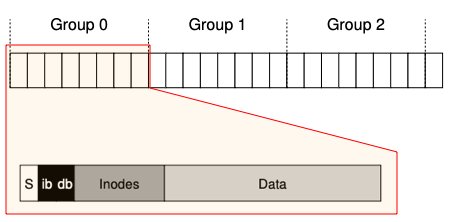
\includegraphics[width=0.8\linewidth]{images/midterm_1_solution_18.png}
    \end{center}
\end{itemize}

\section{Bitmap}

\begin{itemize}
    \item Are excellent way to \underline{manage free space}
    \item tracks whether inodes/data block of the group are allocated
\end{itemize}

\section{FFS Policies: Allocating Files and Directories}

\begin{itemize}
    \item Basic Idea: keep related stuff together, and keep related stuff
    far apart
    \item Directories Step

    \begin{enumerate}[1)]
        \item Find the \textbf{cylinder group} with a low number of allocated directories
        and a high number of free inodes

        \begin{itemize}
            \item low number of allocated directories $\to$ to balance directories
            across groups
            \item high number of free nodes $\to$ to subsequently be able to allocate a bunch offiles
        \end{itemize}
        \item Put directory data and inode to the \textbf{cylinder group}
    \end{enumerate}

    \item Files Step

    \begin{enumerate}[1)]
        \item Allocate the data blocks of a file in the same \textbf{cylinder group} as its inode
        \item Place all files in the same directory in the cylinder group of the directory they are in

        \bigskip

        \underline{\textbf{Example}}

        \bigskip

        On putting \texttt{/a/c}, \texttt{/a/d}, \texttt{/b/f}, FFS would place

        \begin{itemize}
            \item \texttt{/a/c}, \texttt{/a/d} as close as possible in the same \textbf{cylinder group},
            \item \texttt{/b/f} located far away (in some other \textbf{cylinder group})
        \end{itemize}
    \end{enumerate}
\end{itemize}

\section{Inode}

\begin{center}
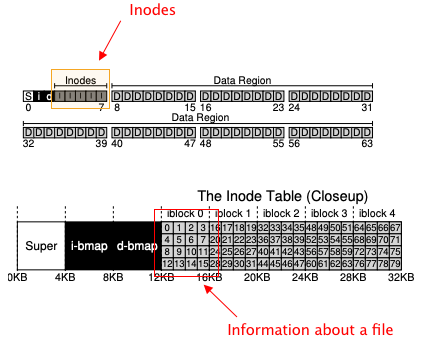
\includegraphics[width=\linewidth]{images/midterm_1_solution_12.png}
\end{center}

\begin{itemize}
    \item Is a short form for \textbf{index node}
    \item Contains disk block location of the object's data $^{[1]}$
    \item Contains all the information you need about a file (i.e. metadata)

    \begin{itemize}
        \item File Type
        \begin{itemize}
            \item e.g. regular file, directory, etc
        \end{itemize}
        \item Size
        \item Number of blocks allocated to it
        \item Protection information
        \begin{itemize}
            \item such as who owns the file, as well as who can access it
        \end{itemize}
        \item Time information
        \begin{itemize}
            \item e.g. When file was created, modified, or last accessed
        \end{itemize}
        \item Location of data blocks reside on disk
    \end{itemize}
\end{itemize}

\section{Crash Consistency}

\begin{itemize}
    \item Goal: How to update persistent data structures despite the presence of
    a \textbf{power loss} or \textbf{system crash}?
\end{itemize}

\section{Crash Scenarios}

\begin{center}
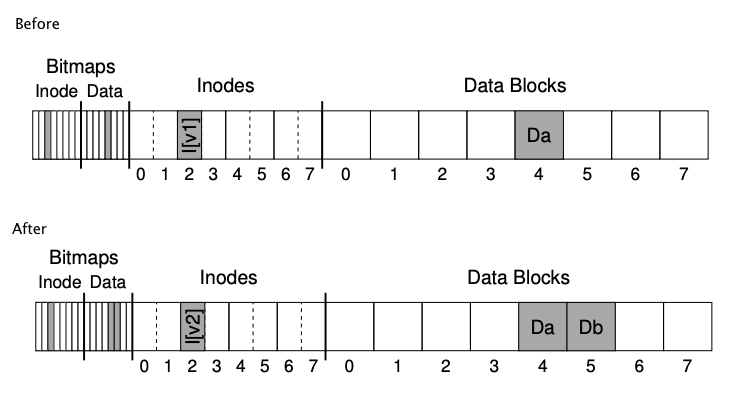
\includegraphics[width=\linewidth]{images/midterm_1_solution_19.png}
\end{center}


\begin{enumerate}[1)]
    \item Just the data block (Db) is written to disk

    \bigskip

    \begin{itemize}
        \item No inode that points to it
        \item No bitmap that says the block is allocated
        \item It is as if the write never occured
        \item There is no problem here. All is well. (In file system's point of view)
    \end{itemize}

    \bigskip

    \item Just the updated inode (I[v2]) is written to disk

    \bigskip

    \begin{itemize}
        \item Inode points to the disk where \texttt{Db} is about to be written
        \item No bitmap that says the block is allocated
        \item No \texttt{Db} is written
        \item Garbage data will be read
        \item Also creates \textbf{File-system Inconsistency}

        \begin{itemize}
            \item Caused by on-disk bitmap telling us Db 5 is not allocated,
            but inode saying it does
        \end{itemize}
    \end{itemize}

    \bigskip

    \item Just the updated bitmap (B[v2]) is written to disk

    \bigskip

    \begin{itemize}
        \item Bitmap indicates tht block 5 is allocated
        \item No inode exists at block 5
        \item Creates \textbf{file-system inconsistency}
        \item Creates \textbf{space-leak} if left as is

        \begin{itemize}
            \item block 5 can never be used by the file system
        \end{itemize}
    \end{itemize}

    \bigskip

    \item Inode (I[v2]) and bitmap (B[v2]) are written to disk, and not data

    \bigskip

    \begin{itemize}
        \item File system metadata is completely consistent (in perspective of file system)
        \item Garbage data will be read
    \end{itemize}

    \bigskip

    \item Inode (I[v2]) and data block (Db) are written, but not the bit map

    \bigskip

    \begin{itemize}
        \item Creates \textbf{file-system inconsistency}
        \item Needs to be resolved before using file system again
    \end{itemize}

    \bigskip

    \item Bitmap (B[v2]) and data block (Db) are written, but not the inode (I[v2])

    \bigskip

    \begin{itemize}
        \item Creates \textbf{file-system inconsistency} between inode and data bitmap
        \item Creates \textbf{space-leak} if left as is
        \begin{itemize}
            \item Inode block is lost for future use
        \end{itemize}
        \item Creates \textbf{data-leak} if left as is

        \begin{itemize}
            \item Data block is lost for future use
        \end{itemize}
    \end{itemize}
\end{enumerate}

\section{External Fragmentation}

\begin{itemize}
    \item Is various free holes that are generated in either your
    memory or disk space. $^{[8]}$
    \item Are available for allocation, but may be too small to be of
    any use $^{[8]}$
\end{itemize}

\section{Internal Fragmentation}

\begin{itemize}
    \item Is wasted space within each allocated block $^{[8]}$
    \item Occurs when more computer memory is allocated than is needed
\end{itemize}

\*section{Extent Based File System}

\begin{center}
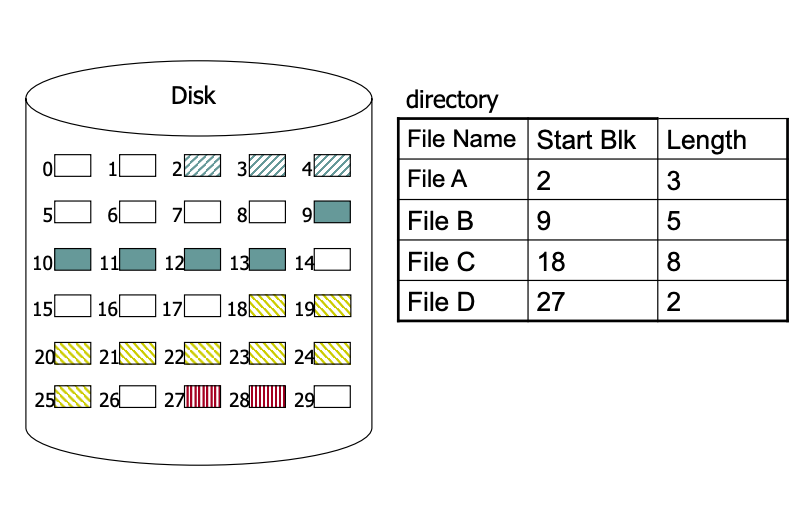
\includegraphics[width=\linewidth]{images/midterm_1_solution_14.png}
\end{center}

\begin{itemize}
    \item Is simply a disk pointer plus a length (in blocks)
    \begin{itemize}
        \item Together, is called \textbf{extent}
    \end{itemize}
    \item Often allows more than one extent
    \begin{itemize}
        \item resolve problem of finding continuous free blocks
    \end{itemize}
    \item Is less flexible but more compact
    \item Works well when there is enough free space on the disk and
    files can be laid out contiguously
\end{itemize}

\bigskip

\underline{\textbf{Example}}

\bigskip

Linux's ext4 file system

\*section{Fields}

\begin{itemize}
    \item Is the members in a structure

    \bigskip

    \begin{center}
    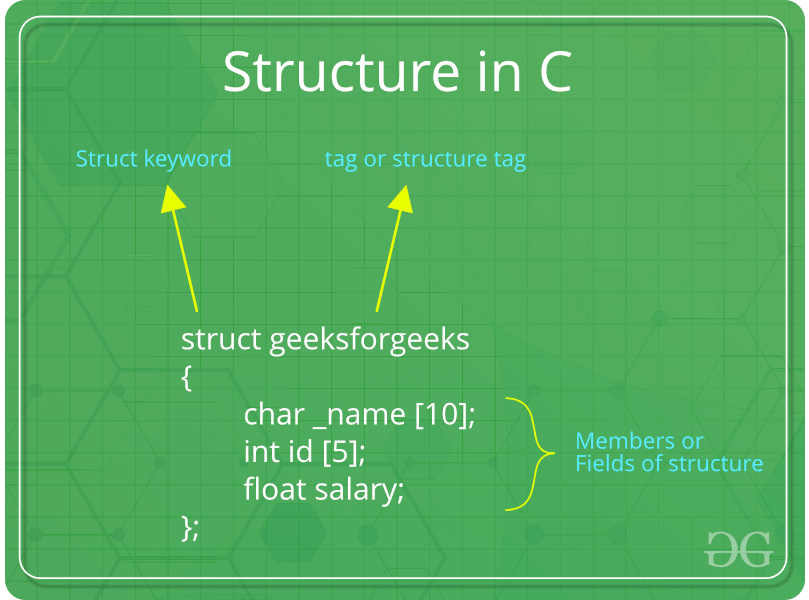
\includegraphics[width=0.6\linewidth]{images/midterm_1_solution_15.png}
    \end{center}
\end{itemize}

\*section{Process List}

\begin{itemize}
    \item Is a data structure in kernel or OS
    \item Contains information about all the processes running in the system
\end{itemize}

\*section{Process Control Block}

\begin{itemize}
    \item Is a data structure in kernel or OS
    \item Contains all information about a process
    \item Is where the OS keeps all of a process' hardware execution state
    \item Generally includes

    \begin{enumerate}[1.]
        \item Process state (ready, running, blocked)
        \item Process number
        \item Program counter: address of the next instruction
        \item CPU Registers: is saved at an interrupt
        \item CPU scheduling information: process priority
        \item Memory management info: page tables
        \item I/O status information: list of open files
    \end{enumerate}
\end{itemize}



\end{document}